\chapter{\label{ch:7-qbo} QBO Teleconnections: the tropical route }

\section{Introduction}


Teleconnections associated with the stratospheric quasi-biennial oscillation (QBO) have been relatively well documented for the stratospheric polar vortex \citep{holton1980,lu2020} and the subtropical jet \citep{garfinkel2011}. The polar and subtropical routes are known to produce surface impacts such as in the North Atlantic \citep{gray2018,andrews2019observed}. 
 Observations have suggested that there is also a tropical route by which the QBO may exhert a significant influence over convetive phenomena such as monsoons \citep{giorgetta1999,liess2012}, the ITCZ \citep{gray2018}, tropical cyclones \citep{gray1984,chan1995} and most recently, the Madden-Julian Oscillation (MJO) \citep{lee2018,wang2019,martin2020jgr}, see section \ref{sq:trop_qbo}. 
 
 Although the polar and subtropical routes of influence of the QBO to the surface are relatively well established, the impact of the QBO over tropical convective remains less well understood for various reasons. First, the short observational record limits the robustness of any analysis that seeks to investigate differences in the state of the tropical atmosphere and oceans between the two QBO phases in a 30-40 yr long dataset. In addition, ENSO variability largely controls the tropical circulation on interannual time-scales, roughly in the same period as the QBO, which makes it difficult to separate the effects of ENSO and the QBO, other than by multi-variable regression analysis as in \cite{gray2018}. As such, studies have struggled to pin-point direct impacts and mechanisms by which the QBO may modulate any aspect of tropical climate. 

Another factor that has hindered the research on this topic has been some difficulties when using GCMs to address QBO tropical teleconnections. 
Modelling work has scarcely analysed these teleconnections in GCMs due to the fact that only recent models are able to reproduce a sufficiently reasonable representation of the QBO, and even so, some of the models in the CMIP6 produce highly unrealistic QBO features \citep{richter2020}. Some of these biases have led several studies to propose the use of nudging experiments where a GCM is relaxed towards an observed or idealized state where the model is forced to reproduce a sensible QBO signal. 

This chapter aims, first, to investigate QBO tropical teleconnections in the pre-industrial control experiments of the MOHC UM: GC3 N96-pi, GC3 N216-pi, UKESM-pi. These simulations are ideal to investigate surface impacts of the QBO because these are very long integrations where external forcing is kept constant within the simulation and the UM is a model that reasonably simulates the QBO characteristics \citep{richter2020}. These simulations are examined first via composite analysis to investigate whether tropical convective phenomena such as the ITCZ and monsoon rainfall show any significant response to the state of the QBO. 

The analysis of the pre-industrial control simulations is followed by a short section that makes the case for the use of nudging experiments using the UM to further investigate the findings of the first section. 
Then, a description of the experimental setup is given and finally, results comparing runs using the nudging technique versus the free running model are presented and discussed in the context of the first section of the chapter. 



\section{Methods and data}

The first part of this chapter focuses on diagnosing the impact of the QBO in CMIP6 experiments. 
However, observational datasets and reanalysis are used to compare the simulated impacts with the short observed response. 
The observational datasets and reanalysis (ERA5) used in this chapter are described in section \ref{sq:obsdata} and consist of the HadSST3 dataset for SST, GPCP for precipitation and ERA5 for the rest of the diagnostics employed in this chapter. 

\subsection{CMIP6 data}

The three pre-industrial control experiments of the MOHC submitted to CMIP6 are used in this chapter: GC3 N96-pi, GC3 N216-pi and UKESM-pi. UKESM-pi and GC3 N96-pi are run with the same resolution (N96) of 1.875$^\circ$x1.25$^\circ$ and GC3 N216-pi is considered a medium-resolution simulation (N216) with atmospheric resolution of 0.83$^\circ$x 0.56$^\circ$. The period of 1850-2350 is used for GC3 N96-pi and GC3 N216-pi and 2050-2650 for the UKESM-pi. 


\subsection{Indices}

The indices for ENSO and the QBO are diagnosed exactly as in section \ref{sq:meth_ch4}, i.e., the 70-hPa zonal mean zonal wind index is used for the QBO with a threshold of 2 m s$^{-1}$ for each phase and the EN3.4 index is used with a threshold of $\pm$0.65 to define positive or negative events.

\section{Teleconnections in the pre-industrial control experiments}

\begin{figure}[b!]
\centering
 %\noindent
 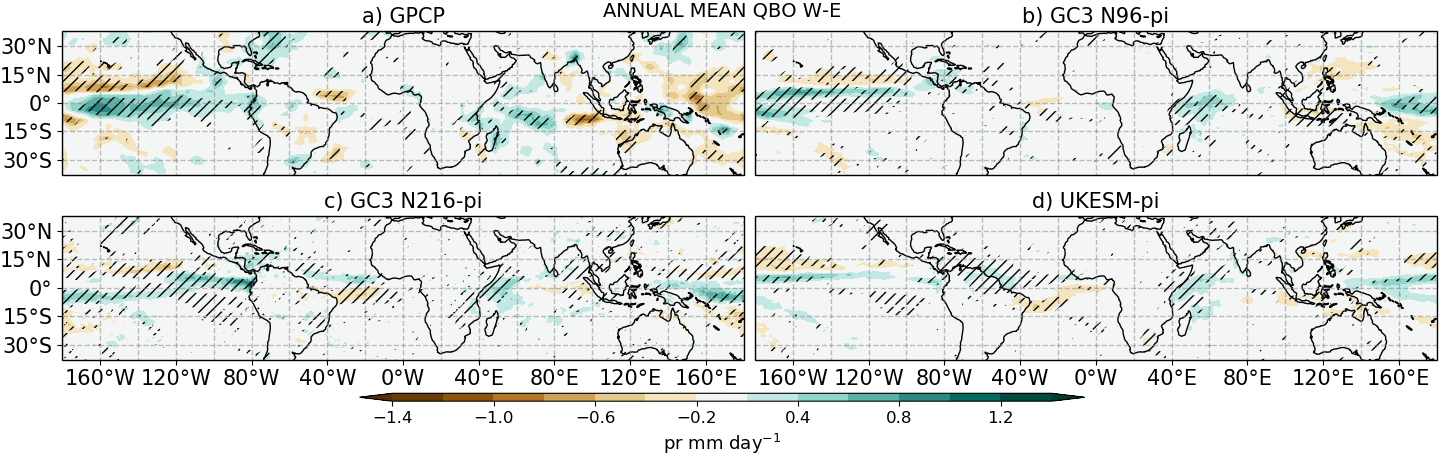
\includegraphics[width=\linewidth]{figures/piprclimqbowqboe.png}
\caption[Annual mean precipitation composite difference QBO W-E ]{ Annual mean precipitation difference between QBO W-E phases in (a) GPCP, (b) GC3 N96-pi, (c) GC3 N216-pi and (d) UKESM-pi. Hatching denotes statistical significance to the 95\% confidence level using bootstrapping with replacement for each composite sample. }
\label{fig:qboclim}
\end{figure}

Surface impacts of the QBO in the tropics have scarcely been investigated in CMIP models, however, recent studies have assessed state-of-the-art CMIP6 models for their representation of the effect of the QBO on the tropopause temperature structure and precipitation \citep{serva2021}.
Their finding suggest that biases in the tropopause layer variability may hinder the representation of QBO effects over tropical convection. 
This point is particularly important as most observational studies argue that the impact of the QBO over tropical tropopause temperatures is the reason for observed impacts in precipitation. The main mechanism proposed via which the QBO could affect convection and precipitation is the change in upper-level static stability associated with the tropopause layer temperature structure variability. 

This section examines more closely how the MOHC piControl experiments simulate the effect of the QBO over seasonal-mean precipitation, monsoons and the ITCZ. 




\subsection{Seasonal variability}

\begin{figure}[b!]
\centering
 %\noindent
 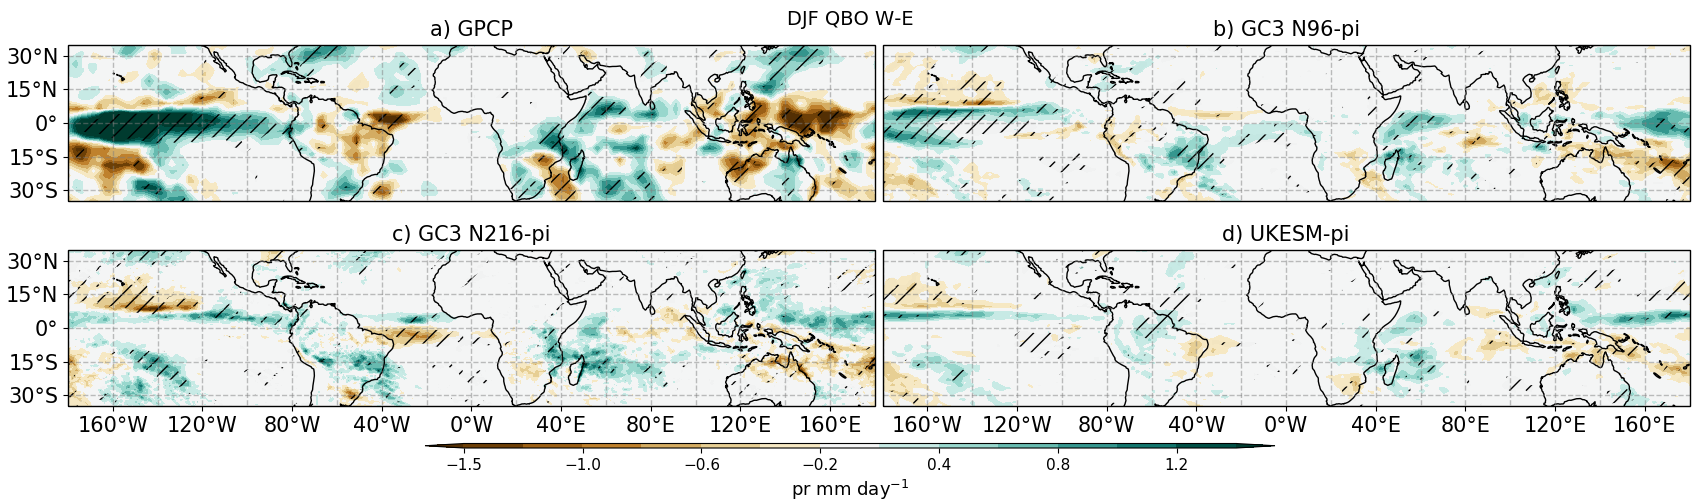
\includegraphics[width=\linewidth]{figures/piprdjfqbowqboe.png}
\caption[DJF mean precipitation composite difference QBO W-E ]{ As in Figure \ref{fig:qboclim} but for DJF. }
\label{fig:qbodjf}
\end{figure}

The difference in the annual mean spatial distribution of precipitation between QBO W and E phases (Figure \ref{fig:qboclim}) shows that the tropical Pacific and the Indian Oceans are the regions where the influence of the QBO is clearer in GPCP. The three simulations agree well with this result, as all three simulations show a positive difference (QBO W-E) in the Central Pacific and the Indian Ocean. However, this pattern although this pattern depicts annual mean differences the impacts of the QBO are more clearly marked over specific seasons. %, and in fact, the pattern exhibits strong seasonal variability. 

For example, during DJF (Figure \ref{fig:qbodjf}), the pattern over the Central Pacific is stronger in GPCP and the simulations. The positive difference in the western Indian Ocean and the South Pacific Convergence Zone is also observed in this season and is significant in all the datasets. GC3 N216-pi shows a significant weakening of the Atlantic ITCZ which seems to agree with GPCP, whereas UKESM-pi and GC3 N96-pi show little and unsignificant responses in the same region.
The response in the East Pacific during DJF matches the results of \cite{serva2020}.
%had been previously 


\begin{figure}[t!]
\centering
 %\noindent
 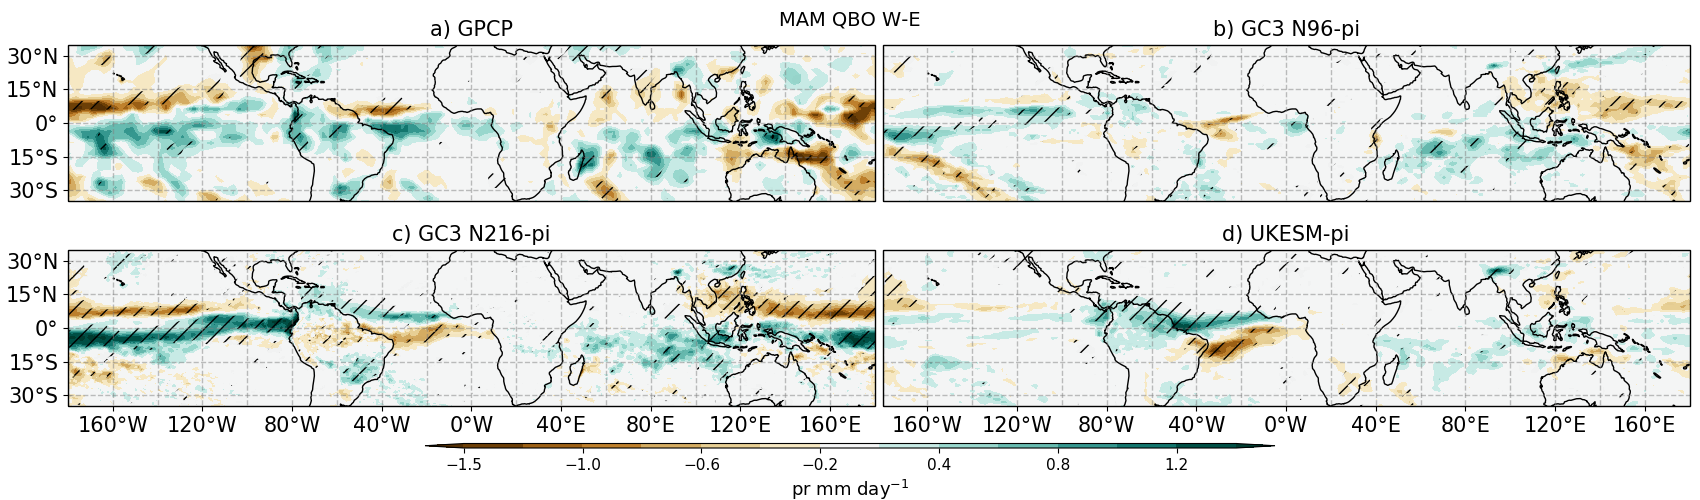
\includegraphics[width=\linewidth]{figures/piprmamqbowqboe.png}
\caption[MAM mean precipitation composite difference QBO W-E ]{ As in Figure \ref{fig:qboclim} but for MAM. }
\label{fig:qbomam}
\end{figure}

During MAM, the strongest response arises in the East Pacific and Atlantic ITCZ regions. In GC3 N216-pi the East Pacific ITCZ is shifted southwards whereas in the Atlantic the ITCZ shows a northward shift. UKESM-pi agrees with the northward shift of the Atlantic ITCZ and exhibits also a strong positive response over northern South America. Although the impact of the QBO over the ITCZ position has been previously described \citep{gray2018,serva2020}, less is known about the specific mechanisms leading to the change in position and strength of the ITCZ. 


\begin{figure}[t!]
\centering
 %\noindent
 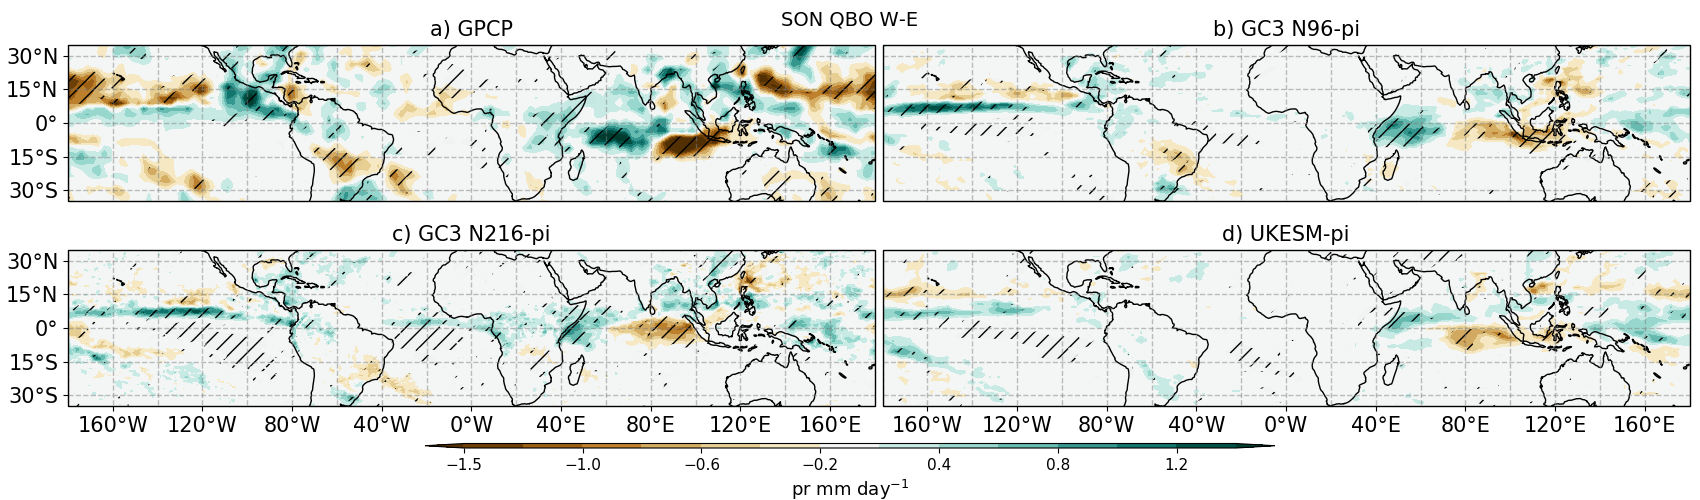
\includegraphics[width=\linewidth]{figures/piprsonqbowqboe.png}
\caption[SON mean precipitation composite difference QBO W-E ]{ As in Figure \ref{fig:qboclim} but for SON. }
\label{fig:qboson}
\end{figure}


In boreal fall (Figure \ref{fig:qboson}), all datasets show a strong and significant indication that the QBO influences the Indian Ocean Dipole (IOD), characterized by a positive difference in the western Indian Ocean and a negative difference in the eastern part in all the datasets. In addition, GC3 N96-pi and GC3 N216-pi show the same response in the Central eastern Pacific as in the other seasons, characterized by a positive and significant response at about 10$^\circ$N.



\begin{figure}[t!]
\centering
 %\noindent
 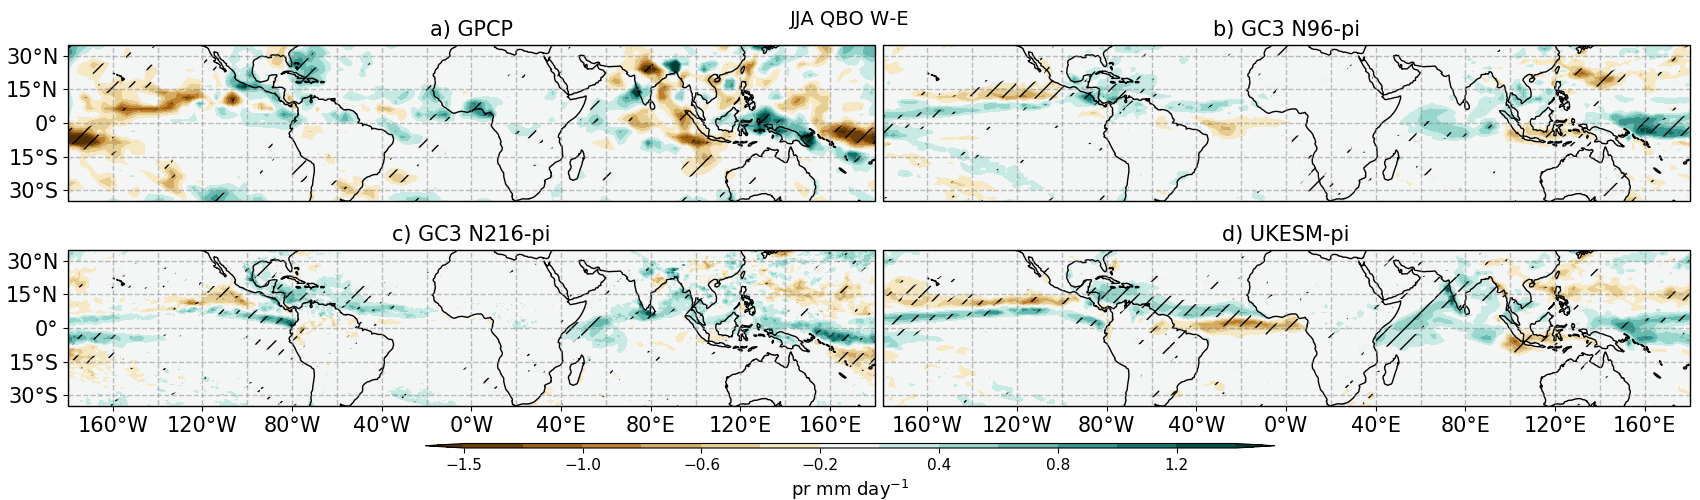
\includegraphics[width=\linewidth]{figures/piprjjaqbowqboe.png}
\caption[JJA mean precipitation composite difference QBO W-E ]{ As in Figure \ref{fig:qboclim} but for JJA. }
\label{fig:qbojja}
\end{figure}

Finally, the JJA seasonal mean pattern (Figure \ref{fig:qbojja}) in the simulations shows little coherent and significant responses in GPCP whereas the simulations show responses in the ITCZ regions, as well as in the Indian Ocean and the Caribbean Sea. Specifically, all the piControl experiments suggest a positive and significant response in the Caribbean Sea and the Indian Ocean; the former, likely related to the northward shift of the Atlantic ITCZ observed in the same season particularly in UKESM-pi. West of the Caribbean Sea, in the easternmost Pacific Ocean a seemingly southward shift of the ITCZ is observed with a negative precipitation response on the western coast of Mexico. Note that in most of these Figures, there seems to be little to no significant effects over land in most seasons, however, two exceptions are observed in Figure \ref{fig:qbojja}. 
A positive and significant response over land is observed in southern Mexico and Central America in all three simulations. Another positive and significant response is observed over the Indian monsoon region, although this signal is onlly present in UKESM-pi. 


\begin{figure}[t!]
\centering
 %\noindent
 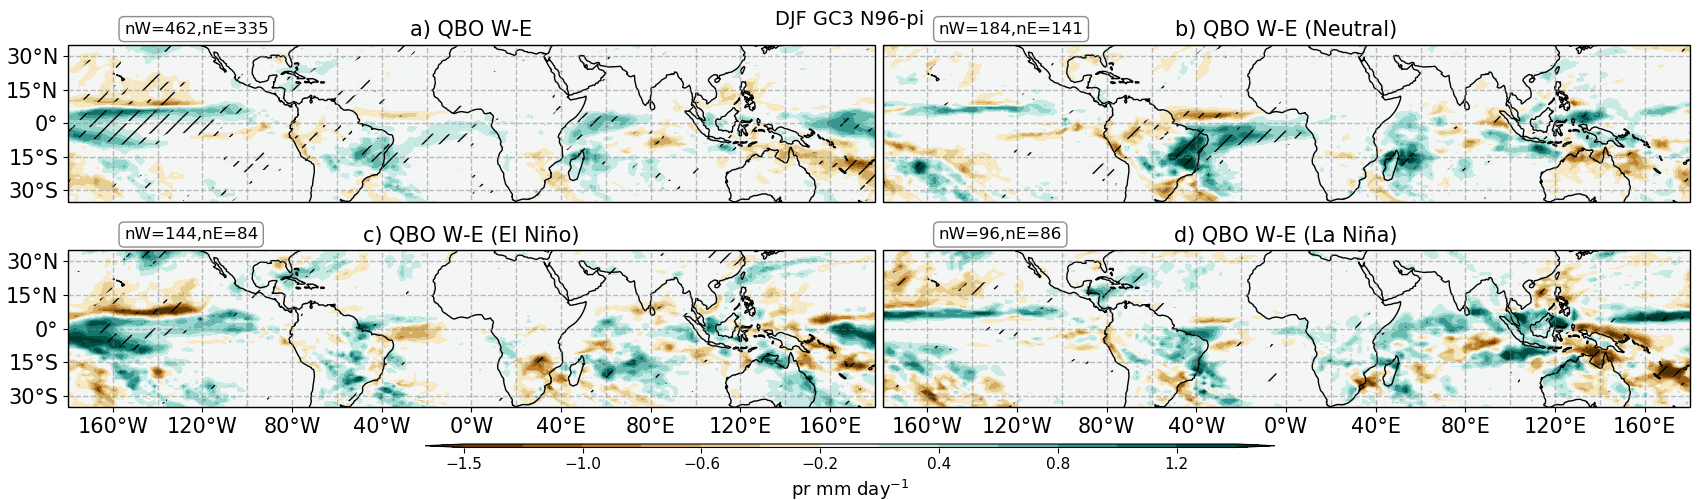
\includegraphics[width=\linewidth]{figures/ensoqboprdjf.png}
\caption[Precipitation response to QBO W-E for GC3 N96-pi under different QBO phases.]{ DJF QBO W-E precipitation differences in GC3 N96-pi for (a) all the events, (b) Neutral ENSO conditions only, (c) El Niño and (d) La Niña conditions. }
\label{fig:qboenso}
\end{figure}

These seasonal mean results consider the influence of the QBO over all possible states of ENSO in each given season. But in observations, either because of sampling uncertainty or an unknown mechanism, ENSO events are predominantly found in given phases of the QBO obscuring these results in the observed record. To what extent, could the state of ENSO modify these seasonal mean results presented in this section is analysed, as a first example, in Figure \ref{fig:qboenso}. 


The pattern in the Central Pacific in the mean DJF response is mainly a result of the difference that arises during ENSO events. The positive response in the Central Pacific in 15$^\circ$S-O is only observed during El Niño events, and the response in this region is rather small during Neutral or La Niña events. In turn, the negative response in the 10$^\circ$N-20$^\circ$N region over the Central Pacific is observed during both la Niña and El Niño seasons but not during Neutral conditions. 
Over the Atlantic ITCZ region and eastern Brazil, the strongest response is observed during Neutral conditions, suggesting that the pattern observed in panel a) is largely a result of Neutral condition seasons. For the rest of the seasons and simulations, this sensivity to the ENSO state is also observed and will be explored in further in the rest of this chapter. 

\begin{figure}[t!]
\centering
 %\noindent
 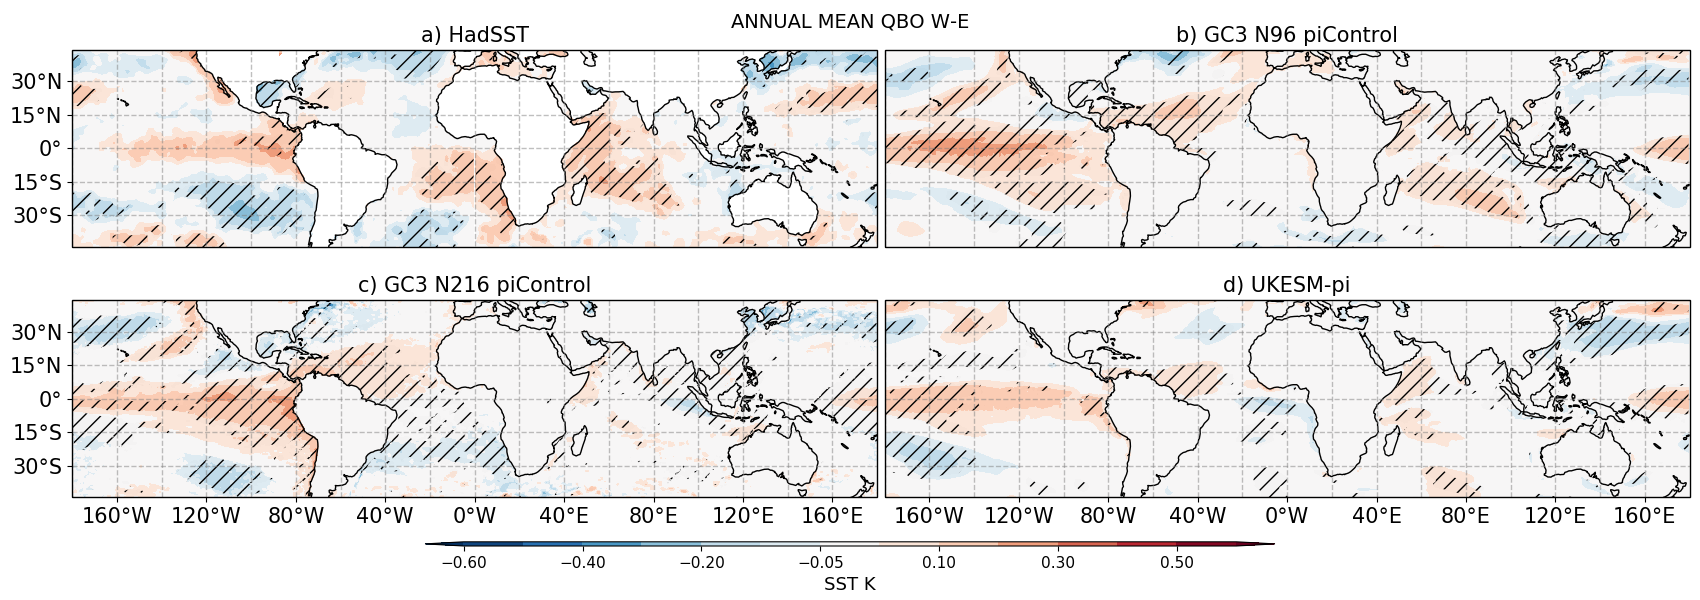
\includegraphics[width=\linewidth]{figures/pisstclimqbowqboe.png}
\caption[Annual mean SST difference QBO W-E under different QBO phases.]{ As in Figure \ref{fig:qboclim} but for SSTs.}
\label{fig:sstclim}
\end{figure}

The simulated and observed responses in the Central Pacific ressemble an El Niño pattern, specially during DJF. In observations, this pattern is likely a result of the increased frequency of El Niño events for the westerly phase than in the easterly phase. 
For this reason, the difference in the annual mean SST pattern is shown (Figure \ref{fig:sstclim}) and evidence of an El Niño pattern is seen as increased SSTs over the Central and Eastern Pacific, even extending to the equatorial Atlantic. 
Although these differences are arguably much weaker than the signal for a typical El Niño event, these differences are significant in all the simulations as well as in the HadSST dataset. 

\begin{figure}[t!]
\centering
 %\noindent
 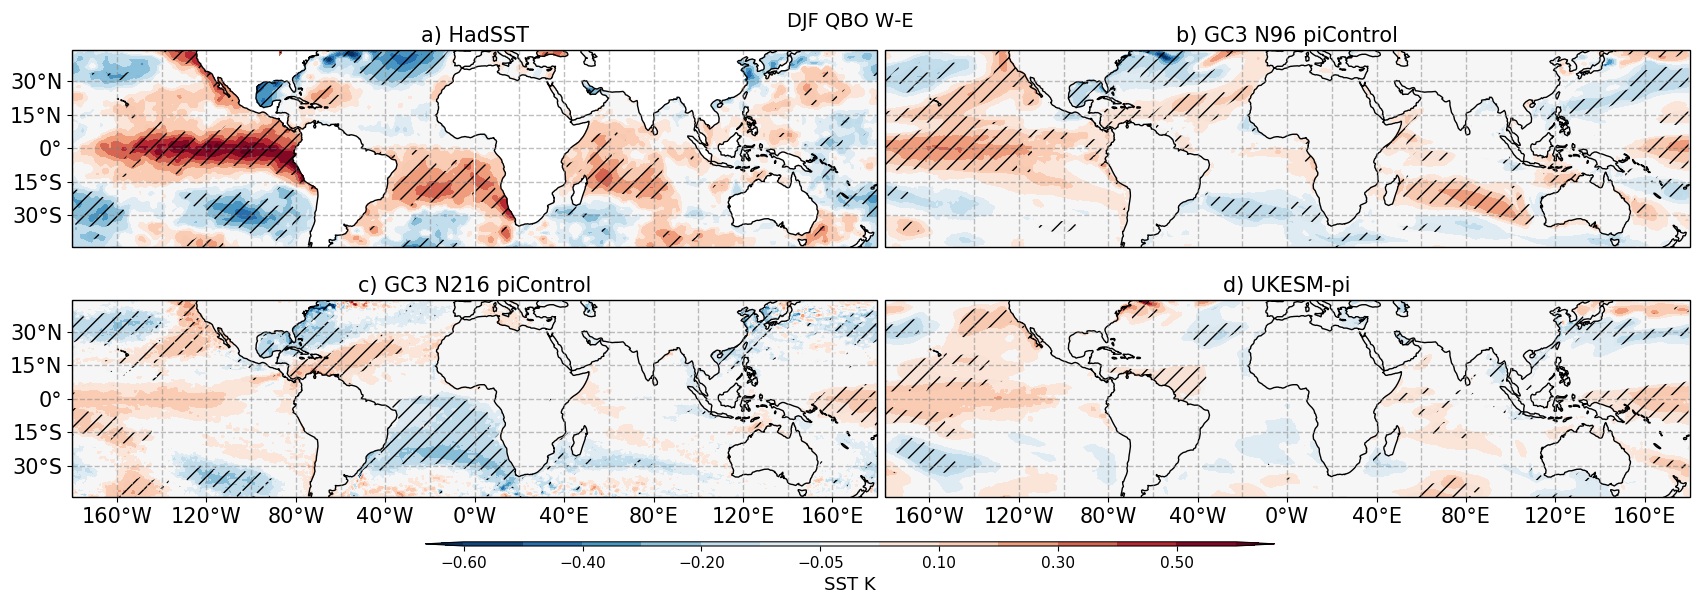
\includegraphics[width=\linewidth]{figures/pisstdjfqbowqboe.png}
\caption[Annual mean SST difference QBO W-E under different QBO phases.]{ As in Figure \ref{fig:qboclim} but for SSTs.}
\label{fig:djfclim}
\end{figure}

The specific SST pattern for DJF confirms that this response seen in the annual mean difference is mostly coming from the boreal winter season, particularly for GC3 N96-pi. The responses in GC3 N96-pi over the North Atlantic and in the Indian Ocean also agree very well with HadSST and are significant. GC3 N216-pi and UKESM-pi also show a positive SST difference over the Central Pacific during DJF although not significant. 
In the case of GC3 N216-pi the strongest SST anomalies over the Central Pacific appear during MAM (not shown) whereas for UKESM-pi the pattern appears during La Niña events with litte-to-no response during other phases of ENSO (not shown). 

This section presented the seasonal mean response in precipitation to the QBO winds at 70 hPa. The main responses observed are the ITCZ shifts over the Pacific and Atlantic Oceans, but significant and robust responses in all the piControl simulations are also observed in the Indian Ocean and the Caribbean Sea.  However, several results require a closer look because during some of these responses arise on very specific months in the long piControl experiments whereas other responses are highly sensitive to the state of ENSO in each season. 
For this reason, the following two sections more closely examine the effect of the QBO over the ITCZs in the East Pacific and Atlantic ITCZs, the Indian Ocean Dipole (IOD) and land-averaged precipitation over monsoon regions. 

\subsection{Impacts over the ITCZ and the monsoons}

\begin{figure}[t!]
\centering
 %\noindent
 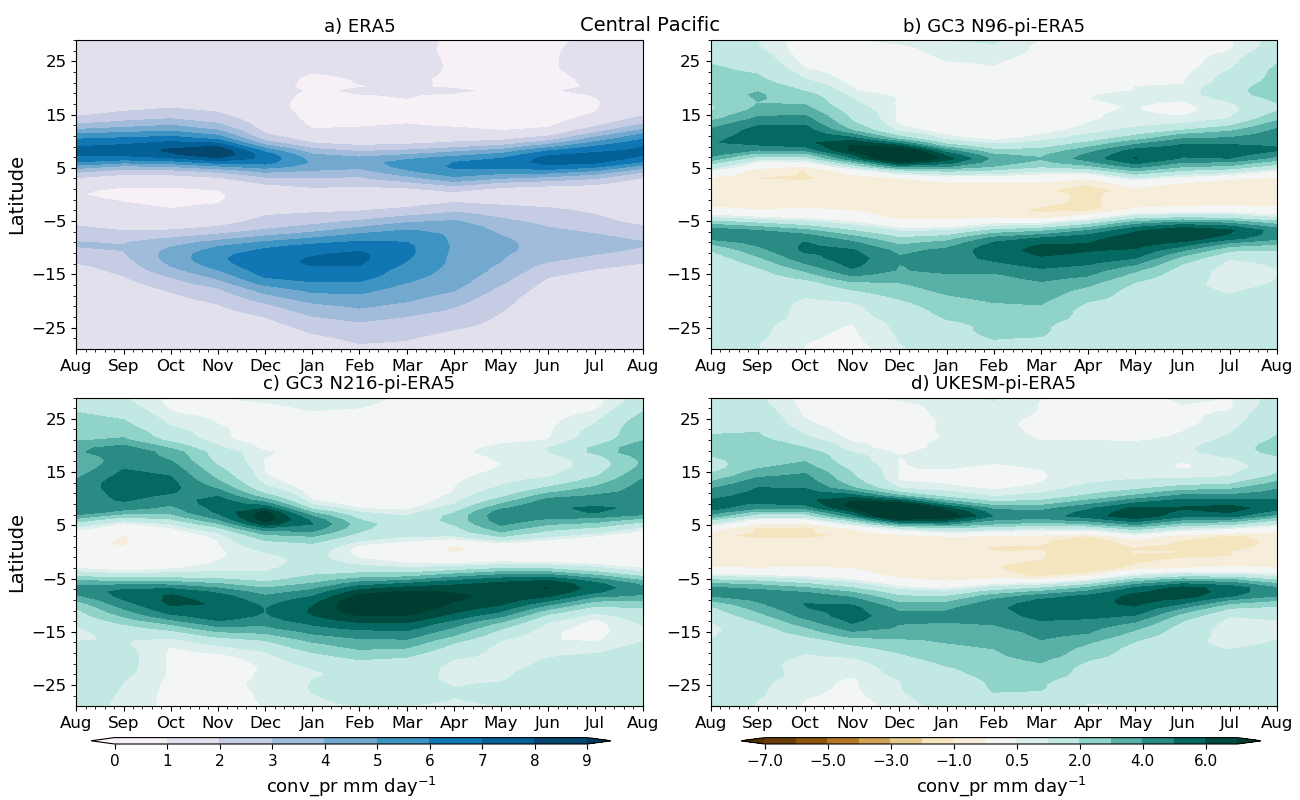
\includegraphics[width=\linewidth]{figures/climcmip_bconv_prcp.png}
\caption[ITCZ seasonal cycle and biases in the Central Pacific.]{Seasonal march of the zonal mean convective precipitation averaged over the Central Pacific sector [180$^\circ$E,200$^\circ$E].}
\label{fig:itczclimcp}
\end{figure}

This section presents the response in the ITCZ position and strength evaluated through the simulated total and convective precipitation in the East Pacific and Atlantic sectors. 
Figures \ref{fig:itczclimcp} and \ref{fig:itczclimatl} show the seasonal march of convective precipitation in the Central Pacific and Atlantic sector in ERA5 and the biases in the three simulations with respect to ERA5. The Atlantic ITCZ in these simulations is not well represented, as shown in previous sections, as the models show a southward bias particularly in DJF. 
In the Central Pacific sector, the models do not show a bias in the position of the ITCZ but rather a bias in the magnitude of convective precipitation, as all the models overestimate the amount of convective precipitation throughout all the seasons. 
 



\begin{figure}[t!]
\centering
 %\noindent
 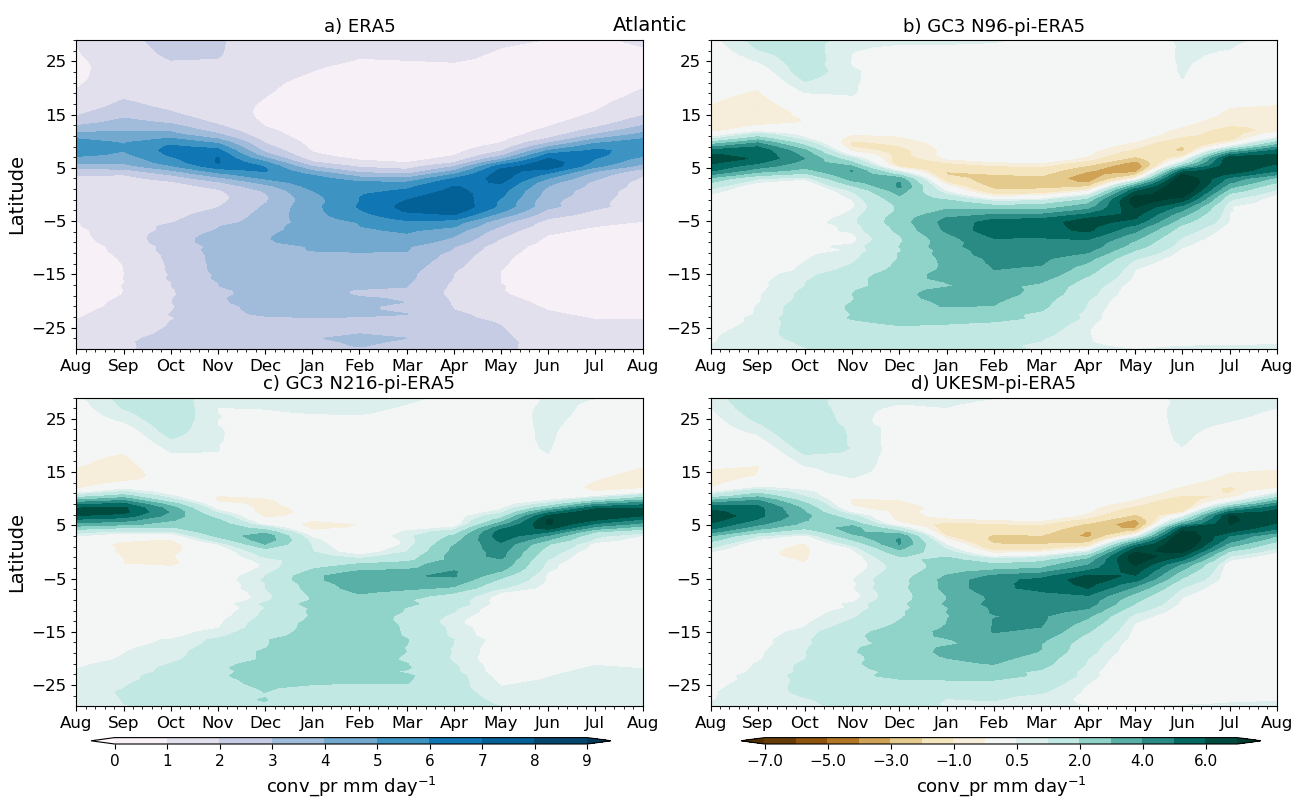
\includegraphics[width=\linewidth]{figures/climcmip_bconv_pratl.png}
\caption[ITCZ seasonal cycle in the Atlantic Sector.]{ As in Figure \ref{fig:itczclimcp}, but for the Atlantic sector [300$^\circ$E,340$^\circ$E]. }
\label{fig:itczclimatl}
\end{figure}

\begin{figure}[t!]
\centering
 %\noindent
 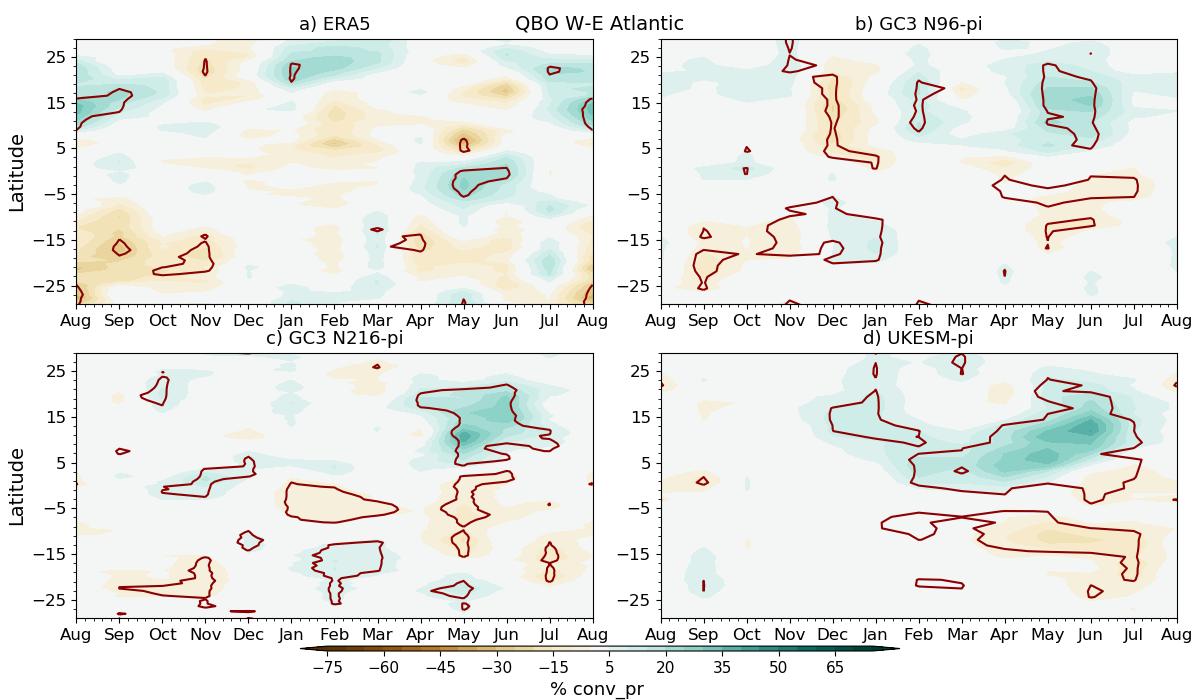
\includegraphics[width=\linewidth]{figures/anomcmip_conv_pratlqbow.png}
\caption[Atlantic ITCZ convective precipitation differences on QBO phase.]{ Zonal mean QBO W-E differences in convective precipitation rates in the Atlantic sector per month, shown as percent (\%) where the difference is weighted by the climatological value at each latitude  and month. The line-contour (red) depict differences that are statistically significant to the 95\% level according to a boostrapping test. }
\label{fig:itczqbowatl}
\end{figure}


\begin{figure}[t!]
\centering
 %\noindent
 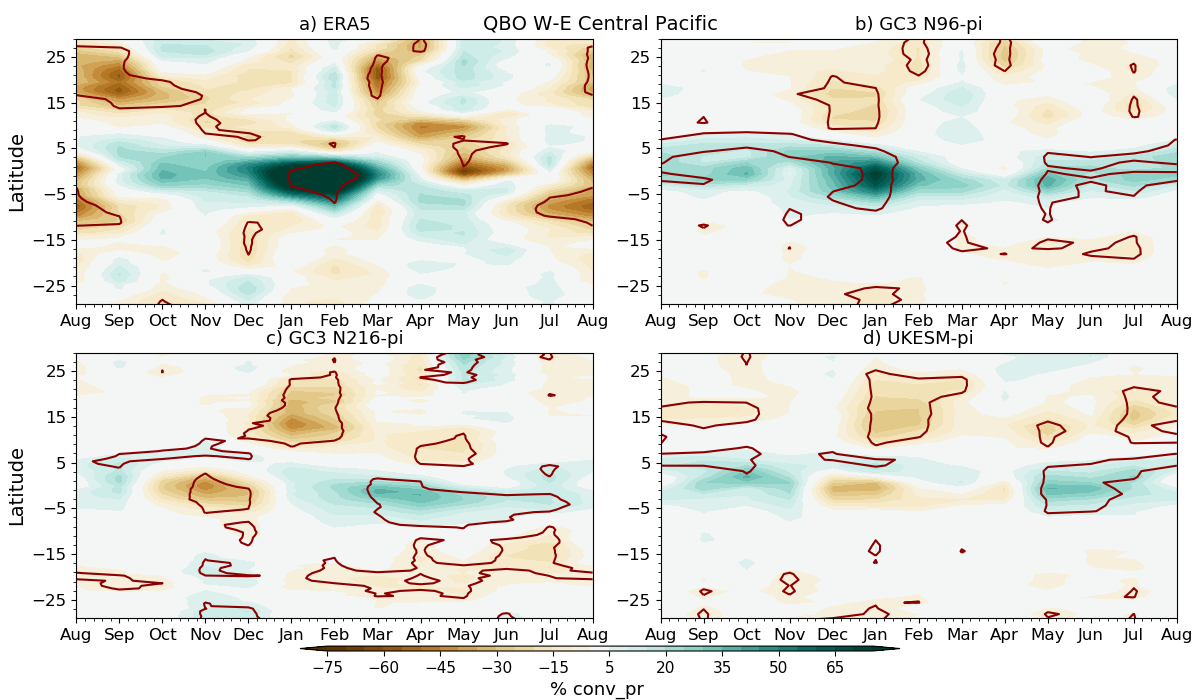
\includegraphics[width=\linewidth]{figures/anomcmip_conv_prcpqbow.png}
\caption[Central Pacific ITCZ convective precipitation differences on QBO phase.]{As in Figure \ref{fig:itczqbowatl} but for the Central Pacific sector.}
\label{fig:itczqbowcp}
\end{figure}

Any effect that the QBO may have on the Atlantic and Pacific ITCZs will be affected by these biases. 
Figures \ref{fig:itczqbowatl} and \ref{fig:itczqbowcp} show the response in convective precipitation to the phase of the QBO in the Atlantic and Pacific sectors. 
The northward shift of the ITCZ during QBO W in the Atlantic sector highlighted in previous sections is confirmed in Figure \ref{fig:itczqbowatl}. In all the simulations, but specially in UKESM-pi there are two significant responses observed from March to July, one positive increase in convective precipitation north of 5$^\circ$N and a corresponding negative difference south of 5$^\circ
$S. The southern negative response is weaker (-20\%) than the positive response north (+40\%). 
The response in ERA5 shows a relatively less robust response, with few significant patterns. % the positive response in August-September 

The southward shift of the ITCZ in the Central Pacific, reported in previous observational studies \citep{gray2018}, is confirmed by Figure \ref{fig:itczqbowcp} which shows that in ERA5 a southward shift of the Central Pacific ITCZ is observed in DJF. 
The simulations agree well with this southward shift, particularly GC3 N96-pi during DJF. However, the simulations show that this southward shift of the ITCZ between QBO phases is also observed in other seasons, for example, from May to September in UKESM-pi and GC3 N96-pi, whereas in GC3 N216-pi the strongest response is seen from February to July.


These results suggest that the response to the phase of the QBO may depend on the climatological representation of the ITCZ position and strength. Nevertheless, these three simulations which exhibit slightly different representations of the ITCZ and the QBO agree on the southward shift of the Pacific ITCZ and the northward shift of the Atlantic ITCZ as the main difference between the westerly and the easterly (W-E) phases of the QBO. 

Although the results in the previous sections showed little-to-no effect of the QBO over tropical precipitation over land, a long record of studies has shown significant responses in observations in the South American, East Asian, Australian and Indian monsoons \citep{giorgetta1999,collimore2003,liess2012,gray2018}. 

%The three simulations 
%\begin{figure}[t!]
%\centering
 %\noindent
% \includegraphics[width=\linewidth]{figures/climcmip_bprep.png}
%\caption[ITCZ seasonal cycle in the Atlantic Sector.]{ As in Figure \ref{fig:itczclimcp}, but for the East Pacific sector [210$^%\circ$E,250$^\circ$E]. }
%\label{fig:itczclimep}
%\end{figure}


\subsection{Interaction with ENSO and teleconnections}

\section{Nudging experiments}



Global climate models exhibit a number of biases in their representation of various aspects of the climate, all of which lead to uncertainty in our ability to make statements about the real-world based on their results. One example of a key bias discussed in this thesis is the magnitude and position of precipitation associated with the ITCZ in the Atlantic Ocean, which is associated with biases in South American precipitation. % the mean state of the Pacific and Atlantic SSTs as well as many others. 
For this section, one relevant bias to consider is how current models represent the tropical stratosphere and, in particular, their representation of the QBO.


The number of GCMs with a full stratosphere have increased notably from CMIP3 to CMIP6 which means that features such as the QBO are increasingly better resolved with each iteration of the CMIP \citep{bushell2020,richter2020}. Nevertheless, several aspects of the QBO are still not well represented by state-of-the-art climate models, such as the period and amplitude of the QBO \citep{schenzinger2017,richter2020}. 
These biases increase uncertainty in teleconnections diagnosed from these models, because these bias may mean that models misrepresent the connections that are observed in the real-world between the tropical stratosphere and other parts of the atmosphere. 

\begin{figure}[t!]
\centering
 %\noindent
 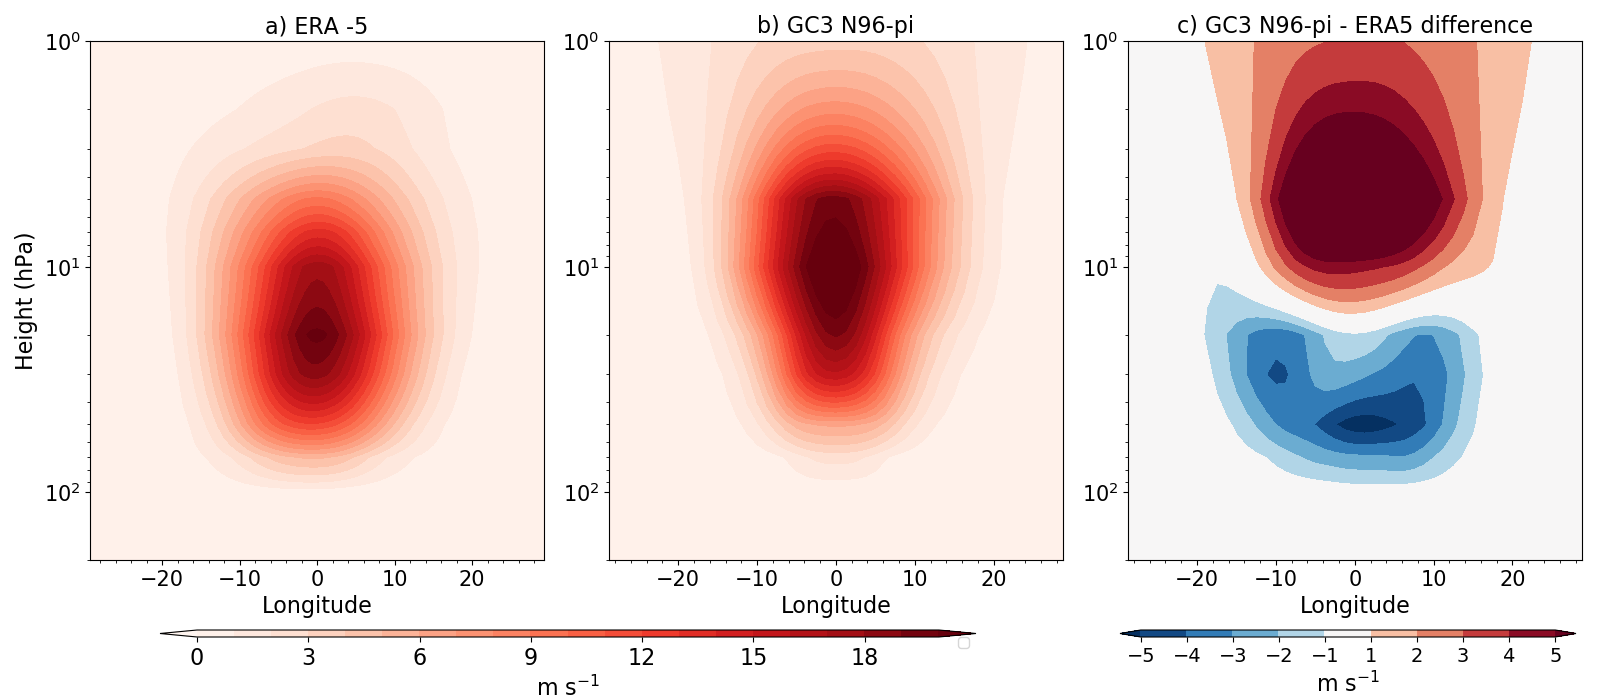
\includegraphics[width=\linewidth]{figures/qboamplitude.png}
\caption[QBO amplitude bias]{Latitude-pressure plot of the amplitude [m s$^{-1}$] of the QBO. Obtained from the zonal mean zonal wind fourier spectrum magnitude within the QBO periods, as in \cite{schenzinger2017}. }
\label{fig:qboamplitude}
\end{figure}

\subsection{The case for nudging}

One key stratospheric bias in most of the existing climate models relates to the representation of the QBO in the lowermost stratosphere. Figure \ref{fig:qboamplitude} illustrates this bias in GC3 N96-pi by comparing the variation of the QBO amplitude  with height and latitude with ERA5; the amplitude is obtained using the method in \cite{schenzinger2017}. The amplitude of the QBO in the lowermost equatorial stratosphere is much smaller and extends to the subtropics less in the model than in ERA5, in agreement previous studies \citep{schenzinger2017,richter2020,bushell2020}. The implication of this bias is that if the QBO signal is too weak in the lower part of the stratosphere in the model, the simulated meridional circulation will also be weaker, and any temperature anomaly associated with this residual circulation will also be smaller near the tropopause. 

The temperature variability in the tropopause layer associated with the QBO is the leading hypothesis \citep[][]{collimore2003,liess2012,nie2015,gray2018} by which the QBO could modulate convection in the tropics. 
Models that simulate a weaker than observed temperature signal near the tropopause associated with the QBO may dampen any tropical effect of the QBO. For this reason, several studies have argued in favour of performing numerical experiments with a GCM where the stratosphere is relaxed towards an observed or idealized state \citep[e.g.][]{lee2018,gray2020,martin2021} to surpass this bias. The purpose of these experiments would be to improve the representation of stratospheric features such as the QBO in order to investigate how accurately representing these stratospheric oscillations can modify impacts elsewhere. 

The following section describes a nudging protocol that was implemented for the second part of this chapter using the Met Office Unified Model. The aim of these experiments is to investigate how the tropical route of QBO teleconnections is modified when the representation of the QBO is improved, and whether nudging is a good tool for this purpose.

\subsection{The nudging protocol}

This section describes the experimental setup for the nudging experiments. 
The GC3.1 configuration of the UM model is used (model version 11.4), using an atmospheric horizontal resolution of N96 (corresponding to the low-resolution version of the simulations of the MOHC submitted to CMIP6). 
Both atmosphere-only and ocean-atmosphere coupled experiments were conducted, in all cases spanning the period 1981-2015, using a present-day climate setup where all forcings are set constant to those of the year 2000, so there is no variation in, e.g., greenhouse gases within these simulations.


\begin{figure}[t!]
\centering
 %\noindent
 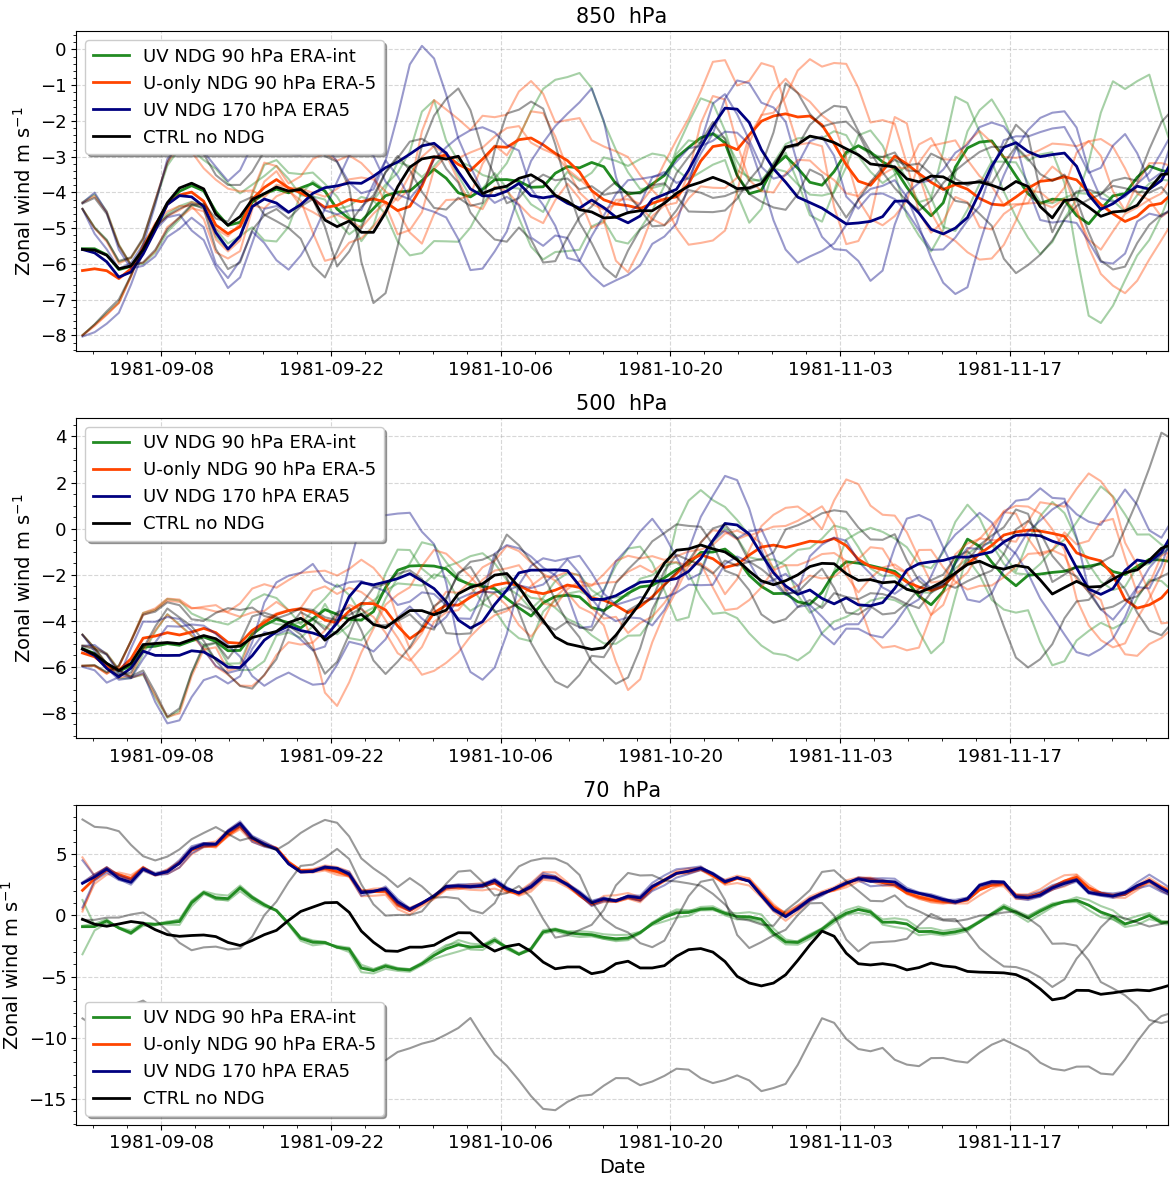
\includegraphics[width=\linewidth]{figures/u_test__.png}
\caption[Time-series of zonal-mean winds under different nudging conditions]{Time-series of the zonal-mean zonal wind in the 10$^\circ$S-10$^\circ$N band at the 850 hPa (upper), 500 (middle) and 70 hPa (lower) levels. Results are from atmosphere-only simulations without nudging (CTRL no NDG), with nudging applied to both $u$ and $v$ up from the 90 hPa level using ERA-interim data (UV NDG 90 hPA ERA-int), with nudging up from 170 hPa nuding $u$ and $v$ using ERA5 data and finally, nudging only $u$ up from 90 hPa level using ERA5 data. For each kind of the simulation, each ensemble member is shown (faint line) and the ensemble mean (solid line) is shown. }
\label{fig:u_nudg_stv}
\end{figure}

Nudging refers to the relaxation of a variable within the model to a specified state, and is a technique that has recently been used for several purposes such as investigating the MJO-QBO relationship in a climate model \citep{martin2021} and the role of the upper stratosphere for forecasting sudden stratospheric warming events \citep{gray2020}.

In the UM setup, three variables can be relaxed, air temperature ($T$) and the zonal and meridional components of the wind ($u$ and $v$). The nudging is applied at each grid-point, in contrast to the setup in other models \citep[e.g.][]{martin2021} where the relaxation is performed in a zonal-mean sense. Furthermore, the nudging can be specified to certain levels within certain longitudes and latitudes using different reanalysis datasets or even idealized states. To find the experimental setup that resulted in an improvement in the representation of the QBO without over constraining the model's climatological state we conducted several sensitivity tests using an atmosphere-only setup to test the effect of nudging all $u$, $v$ and $T$ compared to just one, as well as the model levels and latitudes where the nudging was applied. 


Figure \ref{fig:u_nudg_stv} shows the time-series of the zonal-mean zonal wind at different levels for the different sensitivity experiments performed. Three ensemble members were performed first for a control simulation with no nudging, a simulation where $u$ and $v$ were relaxed towards ERA-interim, and two simulations with ERA5 as the nudging data, one relaxing $u$ only up from 90 hPa and another relaxing $u$ and $v$ up from 170 hPa. 


These results show that in the troposphere (850 hPa) all the ensemble members as they were started from different initial conditions divert towards different states, whereas in the lower stratosphere, the ensemble members of the nudged simulations converge towards a single state. The nudged simulations at the 70 hPa level differ only due to the nudging data, highlighting the differences in the zonal wind in the equatorial stratosphere between ERA5 and ERA-interim. 
From this part on, results using only ERA5 nudging data are presented. 

\begin{figure}[t!]
\centering
 %\noindent
 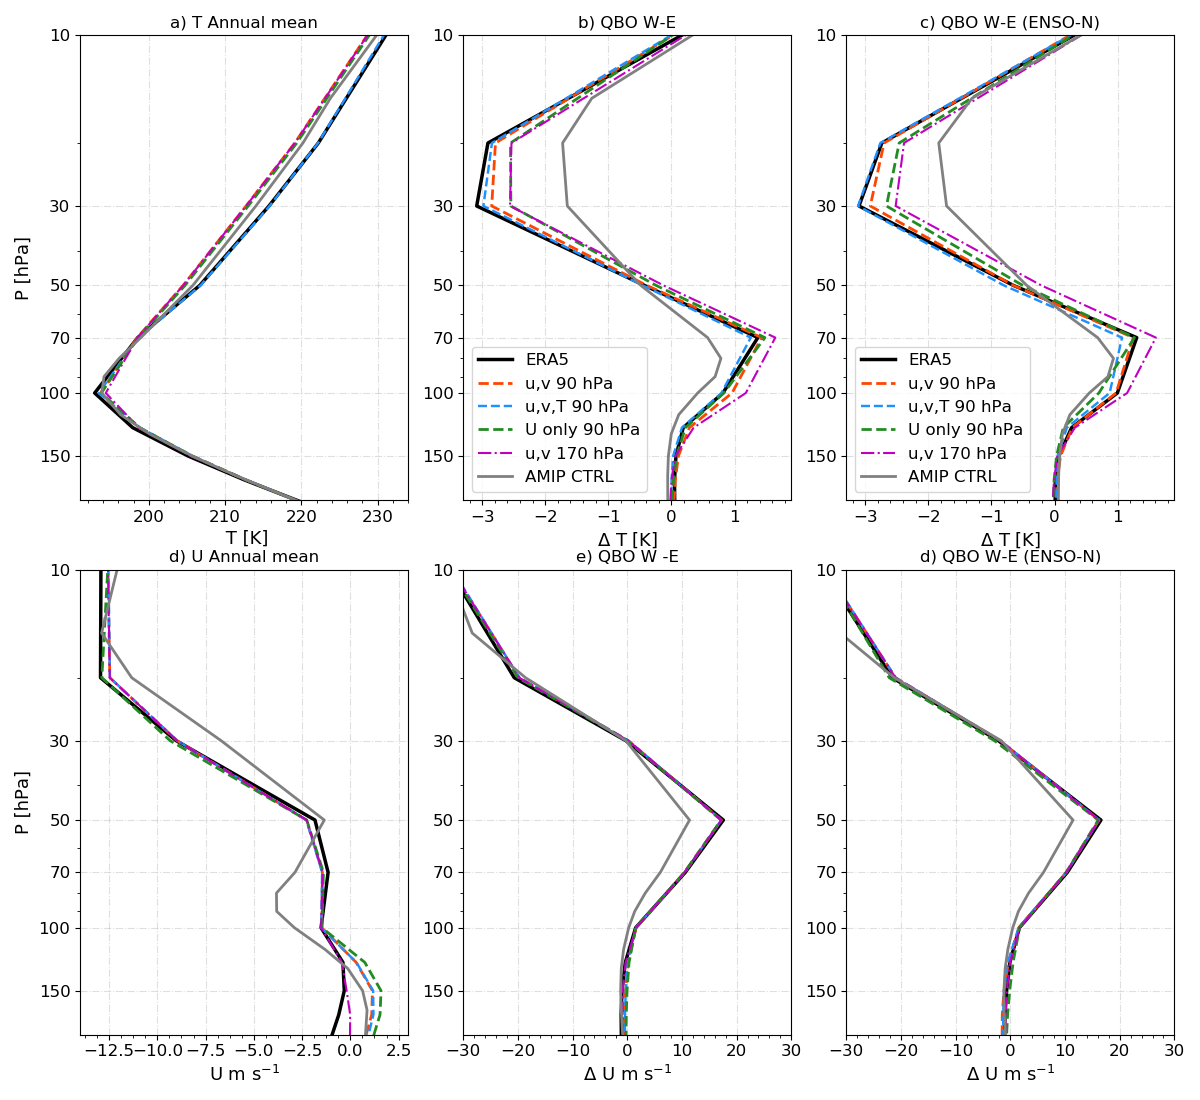
\includegraphics[width=\linewidth]{figures/profilUTclimatology.png}
\caption[Nudging sensitivity QBO profiles]{Vertical profiles of zonal mean temperature (a-c) and zonal wind (d-f) depicting the climatological state (a, d), the QBO W-E difference (b, e) and the QBO W-E difference during Neutral states of ENSO (c, f). In all the simulations with relaxation, the nudging data was ERA5.}
\label{fig:prof_nudg}
\end{figure}

Figure \ref{fig:prof_nudg} shows the vertical profiles of temperature and zonal wind in these simulations. Relaxing only $u$, $v$ or both does not appear to over correct the temperature bias in the model (Fig. \ref{fig:prof_nudg}a) whereas relaxing also $T$ provides an identical climatological state of $T$, as expected. The variability of $T$ associated with the QBO, is fairly well represented by all the nudged simulations, compared to the control simulations, even when $T$ was not relaxed towards ERA5. This results proves that the meridional circulation imposed by the shear imposed when relaxing $u$ is enough to force temperature variability within the model through thermal wind balance, as found in \cite{martin2021}. 

The climatological zonal mean zonal wind and the variability of associated with the QBO (Fig. \ref{fig:prof_nudg}d-f) is much improved in the simulations with nudging, as expected, in the stratosphere. Notably, in the simulations where nudging was applied above 100 hPa, the biases lower down in the stratosphere at 150 hPa remain comparable to those of the control simulation, indicating that nudging the stratosphere does not pose a direct effect over the tropospheric climatological state.

 % and different variables were relaxed. 

The final experimental design chosen was to perform the nudging in the model levels 52-72 which roughly correspond to 90 hPa to 4 hPa, with a tapering of 4 levels, which means that full nudging was only working within levels 56-68. The nudging was done at all longitudes in the latitude band of 10$^\circ$S-10$^\circ$N with a latitudinal tapering of 10 degrees on both sides. Only the zonal component of the wind ($u$) was relaxed, which means that $T$ and $v$ were free running. 


Atmosphere-only and coupled ocean-atmosphere simulations were performed with this nudging setup, with corresponding control simulations in which there was no relaxation of any kind. The atmosphere-only, also referred to as AMIP, experiments were run with observed SSTs from the HadSST dataset, so that means that in the nudged AMIP experiments, both the top and bottom boundaries were constrained to match the observations for each timestep. 
For the nudged experiments several ensemble members were performed, three for the atmosphere-only configuration and six for the coupled ocean-atmosphere configuration. Each ensemble member was initialized from a different ocean/atmosphere initial condition in order to decrease the role that internal variability may have on these simulations. 

\begin{table}[t!]
\begin{tabular}{p{2.3cm}|p{2.3cm}|p{1.73cm}|p{3cm}|p{5cm}}
Setup           & YPeriod    & Ensemble members & Name            & Nudging                                          \\ \hline \hline
Atmosphere-only & 1981-2015 & 3                & AMIP            & ERA5. U-only 90 hPa                              \\
Atmosphere-only & 1981-2015 & 2                & AMIP-Control    & No                                               \\
Atmosphere-only & 1981-2015 & 3                & AMIP-Shifted    & ERA5. U-only, 90 hPa. Relaxation shifted -1 year. \\
Coupled         & 1981-2015 & 6                & Coupled         & ERA5. U-only 90 hPa.                             \\
Coupled         & 1981-2015 & 1                & Coupled Control & No.                                             
\end{tabular}
\end{table}

In addition to the nudged and control coupled and AMIP experiments, we performed another atmosphere-only experiment. In the normal AMIP Nudged experiment, the SST driving data corresponds to the zonal wind in the equatorial stratosphere that was observed in the real-world. To evaluate how the fact that SSTs and zonal winds are in phase, we performed an AMIP Shifted experiment, where the nudging data was shifted with a -1 year lag from the SSTs. In this experiment, e.g., the model year 1997 was run using 1997 SSTs but zonal winds in the stratosphere corresponding to 1996 of ERA5. 

The following section presents the result of nudging in the UM GC3 configuration, first by reporting how the tropical tropopause variability is modified when nudging is applied and then by showing the surface impacts associated with the QBO in the nudged experiments.

\section{The effect of nudging for QBO surface impacts in the tropics}

This section investigates the effect of nudging for the representation of the QBO, the variability in the upper troposphere lower stratosphere (UTLS) associated with the QBO, and ultimately, surface impacts driven by QBO effects on tropical convection. 
First, this section evaluates how nudging modifies the wind and temperature variability in the UTLS region compared to control and CMIP6 simulations.  

\begin{figure}[t!]
\centering
 %\noindent
 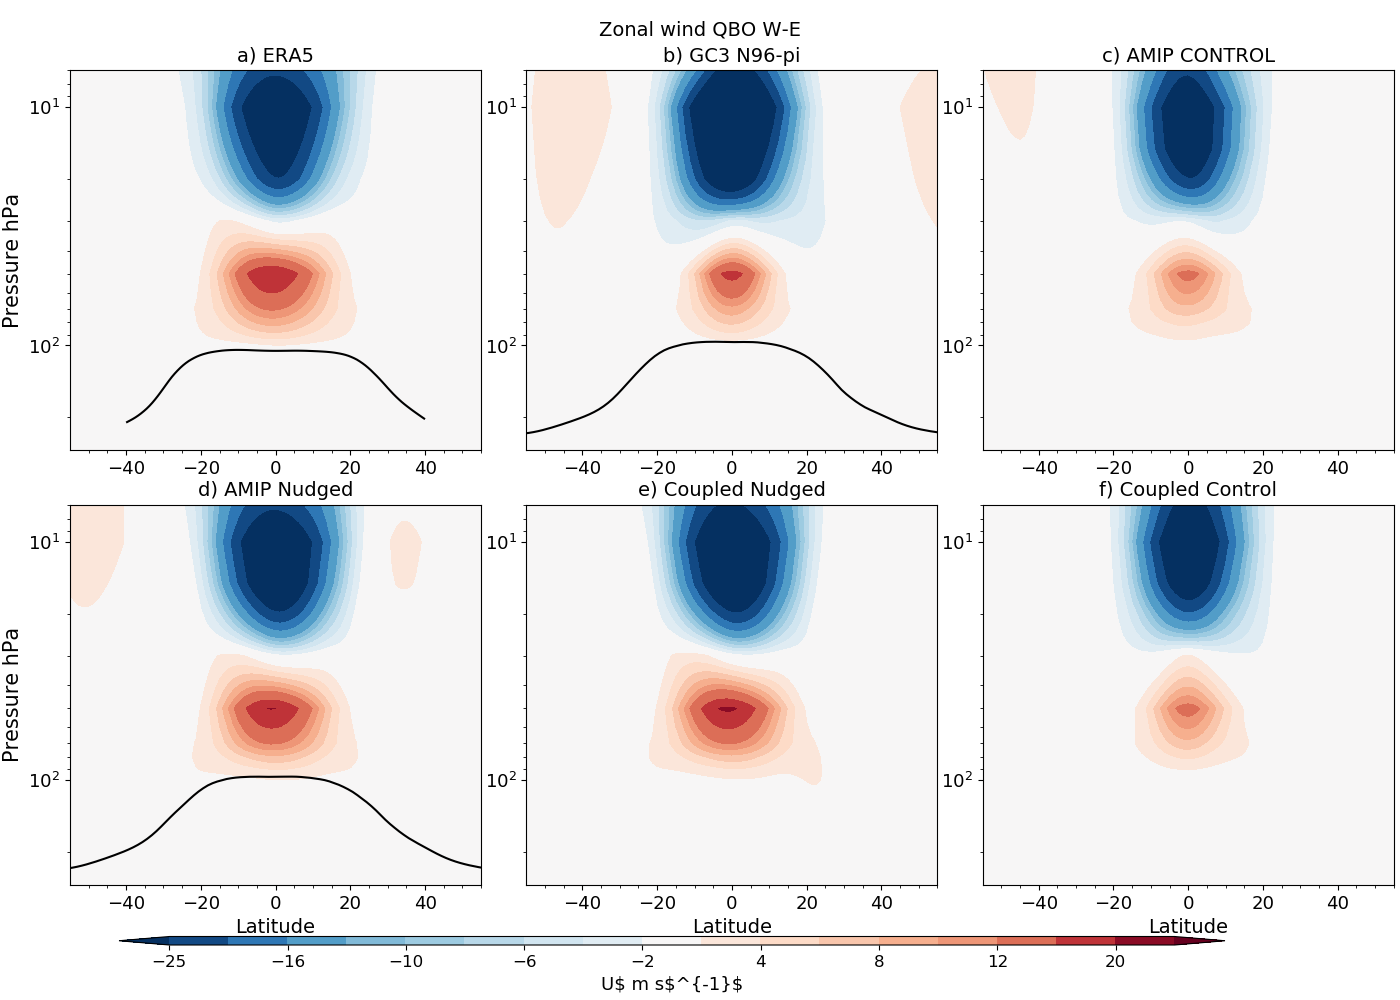
\includegraphics[width=\linewidth]{figures/zonalplotx_wind.png}
\caption[Zonal mean zonal wind QBO difference]{Latitude-height plot of the zonal-mean zonal wind differences (QBO W-E) in (a) ERA5, (b) GC3 N96-pi from CMIP6, the control simulations with no nuding in an (c) AMIP and (f) coupled configurations, and the nudged simulations in (d) AMIP and (e) coupled configurations. The black line denotes the tropopause height obtained from the model data in (b, d) and for ERA5 the tropopause height was found through the gradient threshold method. For the nudged experiments, the ensemble-mean is shown. }
\label{fig:zonal_u}
\end{figure}


\subsection{Tropical UTLS variability}

The nudged experiments aim to replicate the observed variability in the zonal wind leaving the meridional component of the wind and the air temperature to respond freely within the model. 
Figure \ref{fig:zonal_u} shows that the zonal mean difference in zonal wind associated with the QBO phase, in a latitude-height sense, is deficient in the GC3 N96-pi and control experiments, principally near the tropopause as the signal is too narrow and weaker than in the reanalysis. 
The nudging improves this notably and replicates ERA5, as expected since the nudging data is ERA5.  

\begin{figure}[t!]
\centering
 %\noindent
 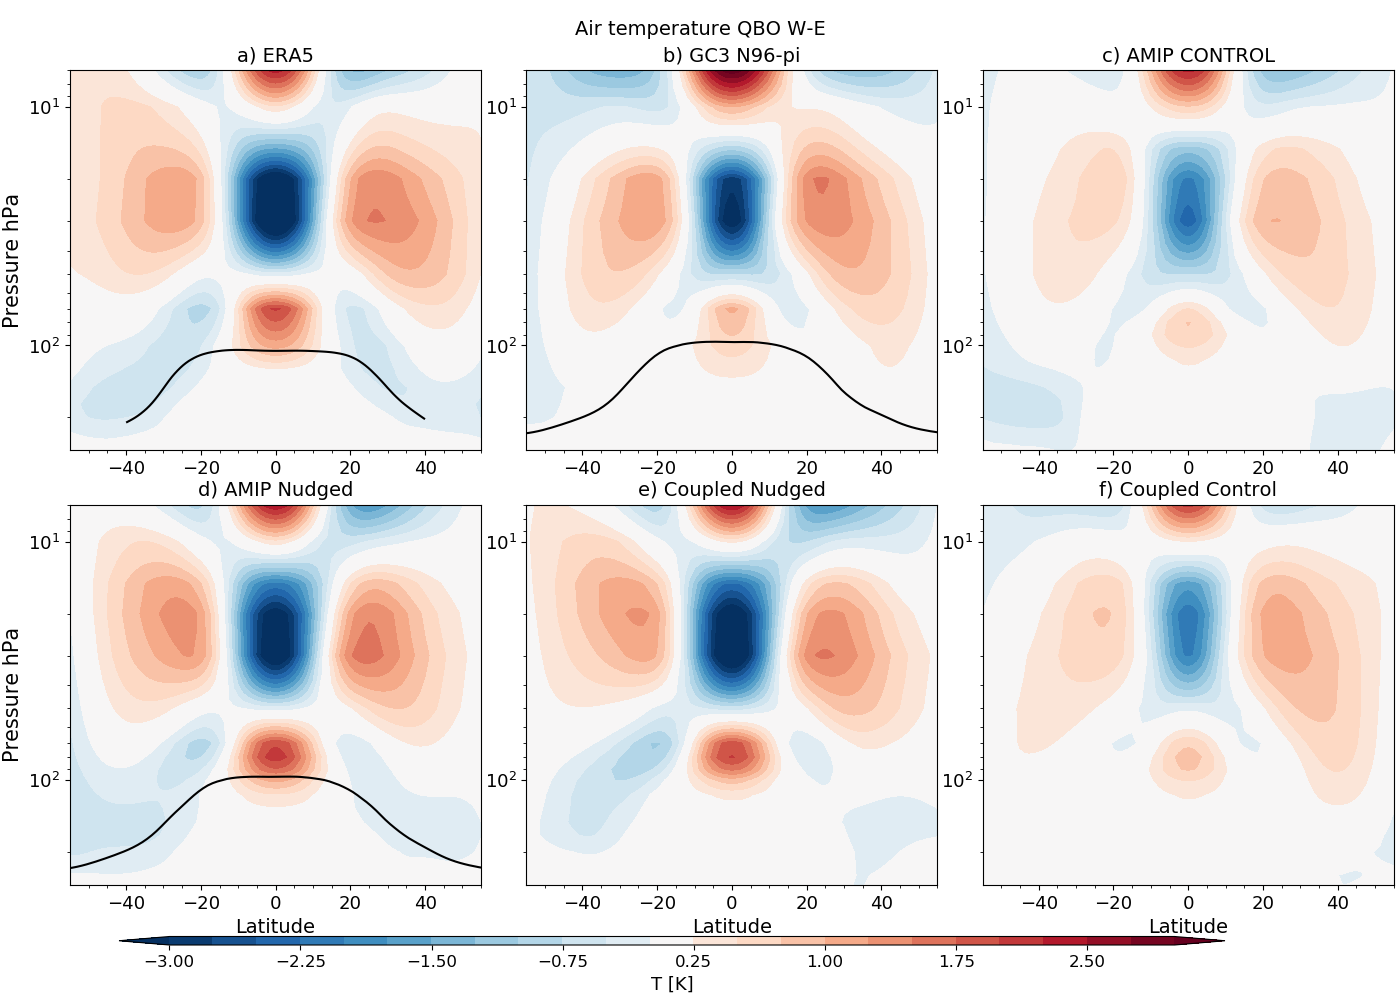
\includegraphics[width=\linewidth]{figures/zonalplotair_temperature.png}
\caption[Zonal mean air temperature QBO difference]{As in Figure \ref{fig:zonal_u} but for air temperature.  }
\label{fig:zonal_T}
\end{figure}

However, the air temperature is free to respond within the model, so Figure \ref{fig:zonal_T} reveals that nudging the zonal wind can also improve the air temperature variability in the lower stratosphere. The positive temperature anomaly in the equatorial region around the 100 hPa at the tropopause level is much weaker in the GC3 N96-pi, AMIP Control and Coupled Control compared to the two nudged experiments and to ERA5. The Nudged experiments not only improve the temperature signal in the equatorial lower stratosphere but seem to overestimate this signal around the 70 hPa level. Furthermore, observations show a horse-shoe temperature anomaly pattern in the subtropics characterised by a negative anomaly that extends from 20-40 degrees north and south, a signal that is missing in the GC3 N96-pi, AMIP Control and Coupled Control experiments but is recovered in the Nudged experiments. This means that without nudging further away than 20 degrees north or south, the subtropical signal is obtained by improving the residual circulation associated with the QBO. 



\subsection{Monsoon rainfall}
